\documentclass[../thesis.tex]{subfiles}
\begin{document}
\chapter{Measuring Triplet Energies}

As discussed in Chapter \ref{sec:excitons}, singlet excitons are typically responsible for molecular emission because the triplet state is quantum mechanically forbidden in the first order approximation.\supercite{Turro1991a}
Emission from the triplet state is allowed with the addition of spin-orbit coupling.\supercite{Baldo1998a}
For applications including OLEDs, solar cells, and organic lasers, spectroscopic characterization of the triplet state is needed, often for molecules where the spin-orbit coupling is weak.\supercite{Tokito2003a,Goushi2004d,Zhang2011a,Schueppel2007}

Most measurements of the triplet energy are conducted via optical pumping.\supercite{Turro1991a,Goushi2004d,Padhye1956,Holmes2003}
However, triplet populations are not generated optically in most materials.\supercite{Turro1991a}
In order for a triplet population to be established, $k_{ISC}$ must be greater than 0.
Additionally, the radiative rate, $k_r$ must be at least competitive with $k_{nr}$.
Since the triplet state is quantum mechanically disallowed without spin-orbit coupling, the radiative rate is typically low compared to the singlet, on the order of $10^6 s^{-1}$.
At room temperature, $k_{nr}$ is often seen be be $10^2-10^6 s^{-1}$.\supercite{Reineke2014}
In order to reduce $k_{nr}$, cryogenic temperatures are often employed, though room-temperateure techniques do exist.\supercite{Reineke2014}

\begin{wrapfigure}{r}{.5\textwidth}
    \begin{minipage}{\linewidth}
    \centering%\captionsetup[subfigure]{justification=centering}
    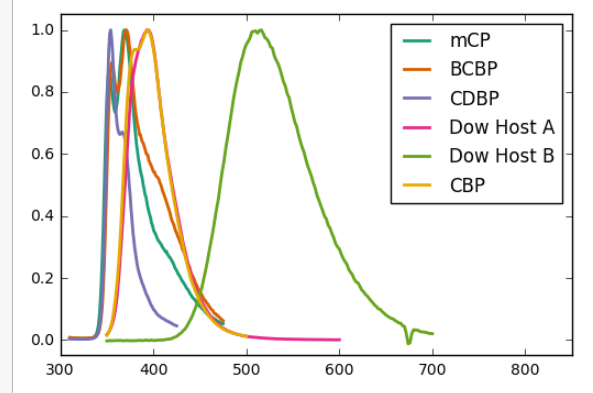
\includegraphics[width=0.48\textwidth]{triplets/fluorescence}
    %\subcaption{}
    %\label{fig:5a}\par\vfill

    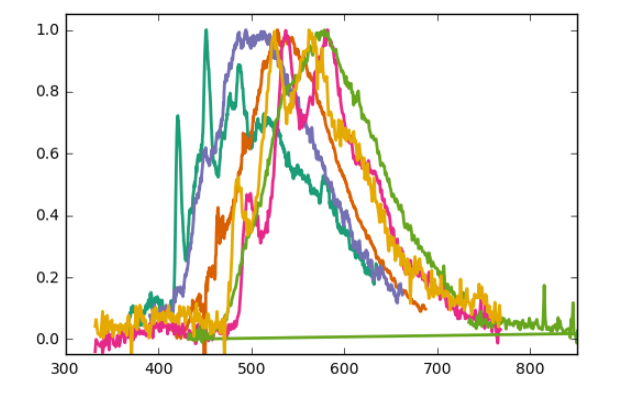
\includegraphics[width=0.48\textwidth]{triplets/phosphorescence}
    %\subcaption{}
    %\label{fig:5b}
\end{minipage}
\caption{Fluorescence (a) and Phosphorescence (b) spectra for several materials obtained from this system.}
\label{fig:triplets}
\end{wrapfigure}

In our lab, I have utilized Janis liquid helium cryogenic optical system to measure triplets.
This takes the temperature to 10K and severely reduces $k_{nr}$
Samples are prepared on Silicon to take advantage of the strong thermal conductivity compared to glass.
If the total emission is collected, the singlet still is far more emissive than the triplet.
However, the difference in their lifetimes can be utilized to seperate them.
Using a pulsed nitrogen laser, the exciton population is exsupercited. 
The singlet population decays quickly, within a few nanoseconds.
However, the triplet lifetime at low temperatures is much longer.
A triggered spectrometer can be used to measure the delayed phosphorescence, and thus measure the triplet emission only.
I have done this with a Princeton Instruments Fergie spectrometer, with a delay of 5ms from the laser pulse.

This system has been used to measure triplet spectra for a variety of materials, shown in Figure \ref{fig:triplets}.
To extract triplet energies, the short wavelength turn on of the triplet spectra can be used.  
This is the highest energy, which seems counter intuitive, but the observed spectra is a decay from $T_1$ to vibrational states of the ground state, $S_0$. 
The triplet energy is defined as the difference between the lowest vibronic of $T_1$ to the lowest vibronic of $S_0$, which is the highest energy transition observed in the spectra.
These spectra show different behavior for sharpness of the leading edge, but a 20\% of the maximum intensity is chosen as the threshold for defining the triplet energy.


\ifcsdef{mainfile}{}{\bibliography{../library}}
\end{document}
